%%%%%%%%%%%%%%%%%%%%%%%%%%%%%%%%%%%%%%%%%%%%%%%%%%%%%%%%%%%%%%%%%%%%%%%%%%%%%%%
%                       CARREGA DE LA CLASSE DE DOCUMENT                      %
%                                                                             %
% Les opcions admissibles son:                                                %
%      12pt / 11pt            (cos dels tipus de lletra; no feu servir 10pt)  %
%                                                                             %
% catalan/spanish/english     (llengua principal del treball)                 %
%                                                                             % 
% french/italian/german...    (si necessiteu fer servir alguna altra llengua) %
%                                                                             %
% listoffigures               (El document inclou un Index de figures)        %
% listoftables                (El document inclou un Index de taules)         %
% listofquadres               (El document inclou un Index de quadres)        %
% listofalgorithms            (El document inclou un Index d'algorismes)      %
%                                                                             %
%%%%%%%%%%%%%%%%%%%%%%%%%%%%%%%%%%%%%%%%%%%%%%%%%%%%%%%%%%%%%%%%%%%%%%%%%%%%%%%

\documentclass[11pt,spanish,listoffigures,listoftables]{tfgetsinf}

%%%%%%%%%%%%%%%%%%%%%%%%%%%%%%%%%%%%%%%%%%%%%%%%%%%%%%%%%%%%%%%%%%%%%%%%%%%%%%%
%                     CODIFICACIO DEL FITXER FONT                             %
%                                                                             %
%    windows fa servir normalment 'ansinew'                                   %
%    amb linux es possible que siga 'latin1' o 'latin9'                       %
%    Pero el mes recomanable es fer servir utf8 (unicode 8)                   %
%                                          (si el vostre editor ho permet)    % 
%%%%%%%%%%%%%%%%%%%%%%%%%%%%%%%%%%%%%%%%%%%%%%%%%%%%%%%%%%%%%%%%%%%%%%%%%%%%%%%

\usepackage[utf8]{inputenc} 

%%%%%%%%%%%%%%%%%%%%%%%%%%%%%%%%%%%%%%%%%%%%%%%%%%%%%%%%%%%%%%%%%%%%%%%%%%%%%%%
%                        ALTRES PAQUETS I DEFINICIONS                         %
%                                                                             %
% Carregueu aci els paquets que necessiteu i declareu les comandes i entorns  %
%                                          (aquesta seccio pot ser buida)     %
%%%%%%%%%%%%%%%%%%%%%%%%%%%%%%%%%%%%%%%%%%%%%%%%%%%%%%%%%%%%%%%%%%%%%%%%%%%%%%%

\usepackage[style=numeric, backend=biber]{biblatex}
% \usepackage[style=authoryear, backend=biber]{biblatex}
\usepackage{csquotes}
\usepackage{graphicx}
\usepackage{tikz}
\usetikzlibrary{trees}
\addbibresource{tex/latex/tfgetsinf/7.Biblio/bibliography.bib}

%%%%%%%%%%%%%%%%%%%%%%%%%%%%%%%%%%%%%%%%%%%%%%%%%%%%%%%%%%%%%%%%%%%%%%%%%%%%%%%
%                        DADES DEL TREBALL                                    %
%                                                                             %
% titol, alumne, tutor i curs academic                                        %
%%%%%%%%%%%%%%%%%%%%%%%%%%%%%%%%%%%%%%%%%%%%%%%%%%%%%%%%%%%%%%%%%%%%%%%%%%%%%%%

\title{???? ????????? \\
         ?????????????? ? ?????}
\author{Adrián Martínez Martínez}
\tutor{Jon Ander Gómez Adrian}
\curs{2023-2024}

%%%%%%%%%%%%%%%%%%%%%%%%%%%%%%%%%%%%%%%%%%%%%%%%%%%%%%%%%%%%%%%%%%%%%%%%%%%%%%%
%                     PARAULES CLAU/PALABRAS CLAVE/KEY WORDS                  %
%                                                                             %
% Independentment de la llengua del treball, s'hi han d'incloure              %
% les paraules clau i el resum en els tres idiomes                            %
%%%%%%%%%%%%%%%%%%%%%%%%%%%%%%%%%%%%%%%%%%%%%%%%%%%%%%%%%%%%%%%%%%%%%%%%%%%%%%%

\keywords{????, ?????????, ????, ?????????????????} % Paraules clau 
         {?????, ???, ???????????????}              % Palabras clave
         {?????, ????? ?????, ?????????????}        % Key words

%%%%%%%%%%%%%%%%%%%%%%%%%%%%%%%%%%%%%%%%%%%%%%%%%%%%%%%%%%%%%%%%%%%%%%%%%%%%%%%
%                              INICI DEL DOCUMENT                             %
%%%%%%%%%%%%%%%%%%%%%%%%%%%%%%%%%%%%%%%%%%%%%%%%%%%%%%%%%%%%%%%%%%%%%%%%%%%%%%%

\begin{document}

%%%%%%%%%%%%%%%%%%%%%%%%%%%%%%%%%%%%%%%%%%%%%%%%%%%%%%%%%%%%%%%%%%%%%%%%%%%%%%%
%              RESUMS DEL TFG EN VALENCIA, CASTELLA I ANGLES                  %
%%%%%%%%%%%%%%%%%%%%%%%%%%%%%%%%%%%%%%%%%%%%%%%%%%%%%%%%%%%%%%%%%%%%%%%%%%%%%%%

\begin{abstract}
????
\end{abstract}
\begin{abstract}[spanish]
????
\end{abstract}
\begin{abstract}[english]
????
\end{abstract}

%%%%%%%%%%%%%%%%%%%%%%%%%%%%%%%%%%%%%%%%%%%%%%%%%%%%%%%%%%%%%%%%%%%%%%%%%%%%%%%
%                              CONTINGUT DEL TREBALL                          %
%%%%%%%%%%%%%%%%%%%%%%%%%%%%%%%%%%%%%%%%%%%%%%%%%%%%%%%%%%%%%%%%%%%%%%%%%%%%%%%

\mainmatter

%%%%%%%%%%%%%%%%%%%%%%%%%%%%%%%%%%%%%%%%%%%%%%%%%%%%%%%%%%%%%%%%%%%%%%%%%%%%%%%
%                                  INTRODUCCIO                                %
%%%%%%%%%%%%%%%%%%%%%%%%%%%%%%%%%%%%%%%%%%%%%%%%%%%%%%%%%%%%%%%%%%%%%%%%%%%%%%%

\chapter{Introducci\'on}

????? ????????????? ????????????? ????????????? ????????????? ?????????????

\section{Motivaci\'on}

????? ????????????? ????????????? ????????????? ????????????? ????????????? 

\section{Objetivos}

- Uno de los problemas que se encuentran en este tipo de conjuntos de datos de imágenes teídas con Hematoxilina y Eosina es la falta de estandarización en el tinte. Por ello en este trabajo se propone una discretización de las imágenes de forma que cada pixel solo pueda tomar uno de entre ocho posibles valores. Estos valores se asignaran a cada pixel de cada imagen aplicando una clusterización... % TODO

\section{Estructura de la memoria}

????? ????????????? ????????????? ????????????? ????????????? ????????????? 

%\section{Notes bibliografiques} %%%%% Opcional

%????? ????????????? ????????????? ????????????? ????????????? ?????????????

%%%%%%%%%%%%%%%%%%%%%%%%%%%%%%%%%%%%%%%%%%%%%%%%%%%%%%%%%%%%%%%%%%%%%%%%%%%%%%%
%                         CAPÍTULO 1                         %
%%%%%%%%%%%%%%%%%%%%%%%%%%%%%%%%%%%%%%%%%%%%%%%%%%%%%%%%%%%%%%%%%%%%%%%%%%%%%%%

\chapter{Estado del arte}

Hola, es un ejemplo, de cita \textcite{Sitnik2021cocahis} hay un dataset chuli

\section{?? ???? ???? ? ?? ??}

????? ????????????? ????????????? ????????????? ????????????? ?????????????

%%%%%%%%%%%%%%%%%%%%%%%%%%%%%%%%%%%%%%%%%%%%%%%%%%%%%%%%%%%%%%%%%%%%%%%%%%%%%%%
%                         CAPÍTULO 2                         %
%%%%%%%%%%%%%%%%%%%%%%%%%%%%%%%%%%%%%%%%%%%%%%%%%%%%%%%%%%%%%%%%%%%%%%%%%%%%%%%

\chapter{Definición de los Dataset}

????? ????????????? ????????????? ????????????? ????????????? ?????????????

\section{Cáncer de Colón}

\subsection{Unitopatho}

El conjunto de datos Unitopatho, presentado en \cite{Barbano_2021} está formado por 292 imágenes etiquetadas de parches imágenes teñidos con Hematoxilina y Eosina (H\&E). Está destinado a la formación de redes neuronales profundas para la clasificación de pólipos colorrectales y la clasificación de adenmoas.

Las imágenes fueron tomadas a través de un escáner Hamamatsu Nanozoomer S210 con una ampliación de 20x (0.4415 $\mu m/px$) y cada imagen, etiquetada por patólogos expertos, pertenece a un paciente diferente y a una de entre seis clases diferentes:

\begin{table}[!ht]
    \centering
    \begin{tabular}{|l|l|}
    \hline
        \textbf{Etiqueta} & \textbf{Descripción} \\ \hline
        \textbf{NORM} & Tejido normal \\ \hline
        \textbf{HP} & Pólipo hiperplásico \\ \hline
        \textbf{TA.HG} & Adenoma tubular, Displasia de alto grado \\ \hline
        \textbf{TA.LG} & Adenoma tubular, Displasia de bajo grado \\ \hline
        \textbf{TVA.HG} & Adenoma tubulovelloso, Displasia de alto grado \\ \hline
        \textbf{TVA.LG} & Adenoma tubulovelloso, Displasia de bajo grado \\ \hline
    \end{tabular}
    \caption{Etiquetas dataset Unitopatho}
    \label{tab:Unitopatho_labels}
\end{table}




\section{Cáncer de Mama}

\subsection{BreakHis}

\begin{table}[!ht]
    \centering
    \begin{tabular}{|l|l|l|l|}
    \hline
        \textbf{Aumento} & \textbf{Benigno} & \textbf{Maligno} & \textbf{Total} \\ \hline
        \textbf{40X} & 652 & 1,370 & 1,995 \\ \hline
        \textbf{100X} & 644 & 1,437 & 2,081 \\ \hline
        \textbf{200X} & 623 & 1,390 & 2,013 \\ \hline
        \textbf{400X} & 588 & 1,232 & 1,820 \\ \hline
        \textbf{Total} & 2.480 & 5.429 & 7.909 \\ \hline
    \end{tabular}
    \caption{Estructura de imágenes en el set de datos BreakHis}
    \label{tab:BreakHis_1}
\end{table}
\subsection{BRACS}

El conjunto de datos BReAst Carcinoma Subtyping (BRACS), presentado en \cite{brancati2021bracs}, contiene imágenes teñidas con Hematoxilina y Eosina (H\&E), divididas en 547 Whole-Slide-Images (WSIs), 4539 Regiones de Interes (ROIs) extraidas de las WSIs. Cada WSI, y sus respectivas ROIs, están anotadas por el consenso de tres patólogos certificados en diferentes categorías de lesiones. Específicamente, BRACS incluye tres tipos de lesiones: benginas, malignas y atípicas, que a su vez se subdividen en un total de siete categorías.

Las WSI están almacenadas en formato .svs como una pirámide multi-resolución, donde la máxima resolución puede exceder fácilmente los 1000 $\times$ 1000 píxeles. Por otro lado, las ROI corresponde a una región con un aumento del 40$\times$ y su resolución puede exceder de los 4000$\times$4000 píxeles.

Ambos grupos de imágenes tienen el mismo tipo de agrupación, en el que las imágenes se separan en tres grandes grupos, BT -tumores benignos-, AT -tumores atípicos- y MT --tumores malignos-. 

El grupo BT contiene muestras de los tipos N, para muestra normal, PB para las muestras patológicamente Benignas, y UDH para muestras con Hiperplasia Ductal Usual.

El grupo AT se subdivide, a su vez, dos grupos. Por un lado el grupo FEA para la Atipia Epitelial Plana (\textit{Flat Epithelial Atypia}) y ADH para la Hiperplasia Ductal Atípica (\textit{Atypical Ductal Hyperplasia}).

Por último, el grupo MT se divide en dos subconjuntos, que incluyen muestras anotadas como Carcinoma Ductal in Situ (DCIS,  \textit{Ductal Carcinoma in Situ}), y Carcinoma Invasivo (IC, \textit{Invasive Carcinoma}).

% \begin{figure}
%     \centering
%     \includegraphics[width=\textwidth]{tex/latex/tfgetsinf/3.Datasets/img/BRACS_Diagram.png}
%     \caption{Organización de grupos del conjunto de datos BRACS}
%     \label{fig:BRACS_Diagram_B}
% \end{figure}


\begin{figure}[h]
\centering
    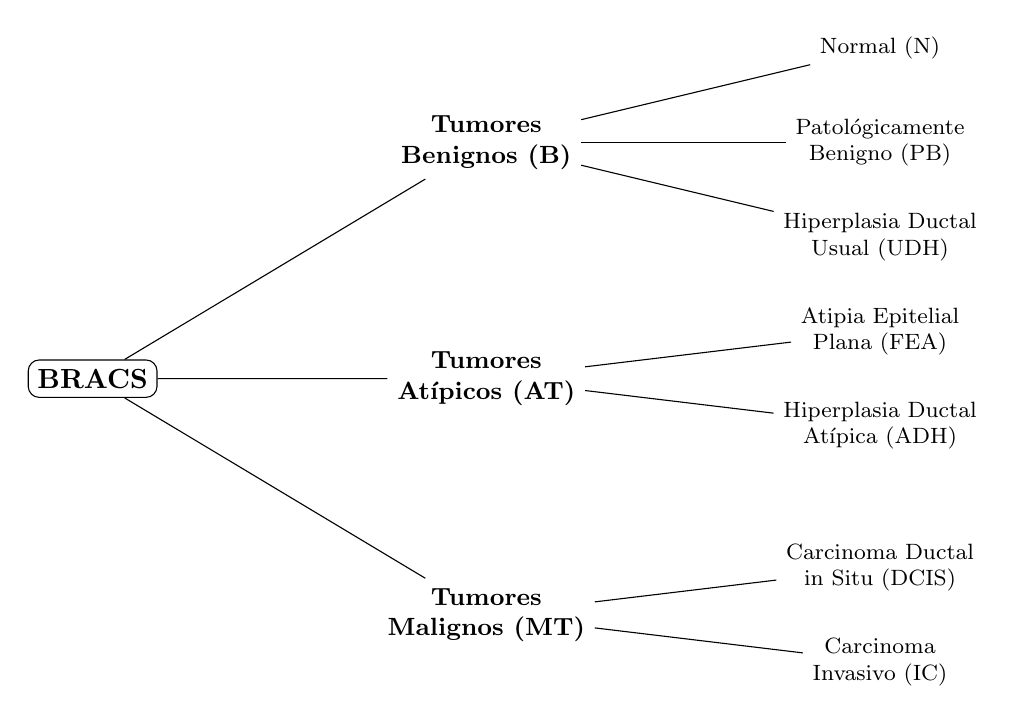
\begin{tikzpicture}[grow=right, level distance=5cm,
    level 1/.style={sibling distance=3cm},
    level 2/.style={sibling distance=1.2cm}]
    \node [rectangle, draw, rounded corners, font=\bfseries] {BRACS}
      child {node[font=\bfseries\small, align=center] {Tumores\\Malignos (MT)}
        child {node[font=\footnotesize, align=center] {Carcinoma\\Invasivo (IC)}}
        child {node[font=\footnotesize, align=center] {Carcinoma Ductal\\in Situ (DCIS)}}}
      child {node[font=\bfseries\small, align=center] {Tumores\\Atípicos (AT)}
        child {node[font=\footnotesize, align=center] {Hiperplasia Ductal\\Atípica (ADH)}}
        child {node[font=\footnotesize, align=center] {Atipia Epitelial\\Plana (FEA)}}}
      child {node[font=\bfseries\small, align=center] {Tumores\\Benignos (B)}
        child {node[font=\footnotesize, align=center] {Hiperplasia Ductal\\Usual (UDH)}}
        child {node[font=\footnotesize, align=center] {Patológicamente\\Benigno (PB)}}
        child {node[font=\footnotesize, align=center] {Normal (N)}}};
    \end{tikzpicture}
    \caption{Organización de grupos del conjunto de datos BRACS}
    \label{fig:BRACS_Diagram}
\end{figure}


\begin{table}[!ht]
    \centering
    \resizebox{\textwidth}{!}{
        \begin{tabular}{|l|l|l|l|l|l|l|l|}
        \hline
                   & \multicolumn{3}{|l|}{\textbf{Group\_BT}}  & \multicolumn{2}{|l|}{\textbf{Group\_AT}} & \multicolumn{2}{|l|}{\textbf{Group\_MT}} \\ \hline
                   & Type\_N & Type\_PB & Type\_UDH & Type\_FEA     & Type\_ADH     & Type\_DCIS     & Type\_IC     \\ \hline
        \textbf{Training}   & 27      & 120      & 56        & 24            & 28            & 40             & 100          \\ \hline
        \textbf{Validation} & 10      & 11       & 9         & 6             & 8             & 9              & 12           \\ \hline
        \textbf{Testing}    & 7       & 16       & 9         & 11            & 12            & 12             & 20           \\ \hline
        \end{tabular}
    }
    \caption{Estructura de imágenes WSI en el set de datos BRACS}
    \label{tab:BRACS_WSI}
\end{table}


\begin{table}[!ht]
    \centering
    \resizebox{\textwidth}{!}{
        \begin{tabular}{|l|l|l|l|l|l|l|l|}
        \hline
                   & \multicolumn{3}{|l|}{\textbf{Group\_BT}}  & \multicolumn{2}{|l|}{\textbf{Group\_AT}} & \multicolumn{2}{|l|}{\textbf{Group\_MT}} \\ \hline
                   & Type\_N & Type\_PB & Type\_UDH & Type\_FEA     & Type\_ADH     & Type\_DCIS     & Type\_IC     \\ \hline
        \textbf{Training}   & 357      & 714      & 389        & 624            & 387            & 665             & 521          \\ \hline
        \textbf{Validation} & 46      & 43       & 46         & 49             & 41             & 40              & 47           \\ \hline
        \textbf{Testing}    & 81       & 79       & 82         & 83            & 79            & 85             & 81           \\ \hline
        \end{tabular}
    }
    \caption{Estructura de imágenes ROI en el set de datos BRACS}
    \label{tab:BRACS_ROI}
\end{table}


%%%%%%%%%%%%%%%%%%%%%%%%%%%%%%%%%%%%%%%%%%%%%%%%%%%%%%%%%%%%%%%%%%%%%%%%%%%%%%%
%                         CAPÍTULO 3                         %
%%%%%%%%%%%%%%%%%%%%%%%%%%%%%%%%%%%%%%%%%%%%%%%%%%%%%%%%%%%%%%%%%%%%%%%%%%%%%%%

\chapter{Aproximación al problema}

????? ????????????? ????????????? ????????????? ????????????? ?????????????


\section{?? ???? ???? ? ?? ??}

????? ????????????? ????????????? ????????????? ????????????? ?????????????

%%%%%%%%%%%%%%%%%%%%%%%%%%%%%%%%%%%%%%%%%%%%%%%%%%%%%%%%%%%%%%%%%%%%%%%%%%%%%%%
%                         CAPÍTULO 4                         %
%%%%%%%%%%%%%%%%%%%%%%%%%%%%%%%%%%%%%%%%%%%%%%%%%%%%%%%%%%%%%%%%%%%%%%%%%%%%%%%

\chapter{Experimentación y resultados}

????? ????????????? ????????????? ????????????? ????????????? ?????????????

\section{?? ???? ???? ? ?? ??}

????? ????????????? ????????????? ????????????? ????????????? ?????????????



%%%%%%%%%%%%%%%%%%%%%%%%%%%%%%%%%%%%%%%%%%%%%%%%%%%%%%%%%%%%%%%%%%%%%%%%%%%%%%%
%                                 CONCLUSIONS                                 %
%%%%%%%%%%%%%%%%%%%%%%%%%%%%%%%%%%%%%%%%%%%%%%%%%%%%%%%%%%%%%%%%%%%%%%%%%%%%%%%

\chapter{Conclusiones}

????? ????????????? ????????????? ????????????? ????????????? ????????????? 

%%%%%%%%%%%%%%%%%%%%%%%%%%%%%%%%%%%%%%%%%%%%%%%%%%%%%%%%%%%%%%%%%%%%%%%%%%%%%%%
%                                BIBLIOGRAFIA                                 %
%%%%%%%%%%%%%%%%%%%%%%%%%%%%%%%%%%%%%%%%%%%%%%%%%%%%%%%%%%%%%%%%%%%%%%%%%%%%%%%

%\begin{thebibliography}{10}

\printbibliography

%%%%%%%%%%%%%%%%%%%%%%%%%%%%%%%%%%%%%%%%%%%%%%%%%%%%%%%%%%%%%%%%%%%%%%%%%%%%%%%
% MODEL D'ARTICLE                                                             %
%%%%%%%%%%%%%%%%%%%%%%%%%%%%%%%%%%%%%%%%%%%%%%%%%%%%%%%%%%%%%%%%%%%%%%%%%%%%%%%
% \bibitem{light}
%    Jennifer~S. Light.
%    \newblock When computers were women.
%    \newblock \textit{Technology and Culture}, 40:3:455--483, juliol, 1999.

%%%%%%%%%%%%%%%%%%%%%%%%%%%%%%%%%%%%%%%%%%%%%%%%%%%%%%%%%%%%%%%%%%%%%%%%%%%%%%%
% MODEL DE LLIBRE                                                             %
%%%%%%%%%%%%%%%%%%%%%%%%%%%%%%%%%%%%%%%%%%%%%%%%%%%%%%%%%%%%%%%%%%%%%%%%%%%%%%%
% \bibitem{ifrah}
%    Georges Ifrah.
%    \newblock \textit{Historia universal de las cifras}.
%    \newblock Espasa Calpe, S.A., Madrid, sisena edició, 2008.

%%%%%%%%%%%%%%%%%%%%%%%%%%%%%%%%%%%%%%%%%%%%%%%%%%%%%%%%%%%%%%%%%%%%%%%%%%%%%%%
% MODEL D'URL                                                                 %
%%%%%%%%%%%%%%%%%%%%%%%%%%%%%%%%%%%%%%%%%%%%%%%%%%%%%%%%%%%%%%%%%%%%%%%%%%%%%%%
% \bibitem{WAR}
%    Comunicat de premsa del Departament de la Guerra, 
%    emés el 16 de febrer de 1946. 
%    \newblock Consultat a 
%    \url{http://americanhistory.si.edu/comphist/pr1.pdf}.

% \end{thebibliography}
\cleardoublepage

%%%%%%%%%%%%%%%%%%%%%%%%%%%%%%%%%%%%%%%%%%%%%%%%%%%%%%%%%%%%%%%%%%%%%%%%%%%%%%%
%                           APÈNDIXS  (Si n'hi ha!)                           %
%%%%%%%%%%%%%%%%%%%%%%%%%%%%%%%%%%%%%%%%%%%%%%%%%%%%%%%%%%%%%%%%%%%%%%%%%%%%%%%

\APPENDIX

%%%%%%%%%%%%%%%%%%%%%%%%%%%%%%%%%%%%%%%%%%%%%%%%%%%%%%%%%%%%%%%%%%%%%%%%%%%%%%%
%                         LA CONFIGURACIO DEL SISTEMA                         %
%%%%%%%%%%%%%%%%%%%%%%%%%%%%%%%%%%%%%%%%%%%%%%%%%%%%%%%%%%%%%%%%%%%%%%%%%%%%%%%

\chapter{Configuració del sistema}

????? ????????????? ????????????? ????????????? ????????????? ?????????????

\section{Fase d'inicialització}

????? ????????????? ????????????? ????????????? ????????????? ?????????????

\section{Identificació de dispositius}

????? ????????????? ????????????? ????????????? ????????????? ?????????????

%%%%%%%%%%%%%%%%%%%%%%%%%%%%%%%%%%%%%%%%%%%%%%%%%%%%%%%%%%%%%%%%%%%%%%%%%%%%%%%
%                               ALTRES  APÈNDIXS                              %
%%%%%%%%%%%%%%%%%%%%%%%%%%%%%%%%%%%%%%%%%%%%%%%%%%%%%%%%%%%%%%%%%%%%%%%%%%%%%%%


\chapter{??? ???????????? ????}

????? ????????????? ????????????? ????????????? ????????????? ????????????? 



%%%%%%%%%%%%%%%%%%%%%%%%%%%%%%%%%%%%%%%%%%%%%%%%%%%%%%%%%%%%%%%%%%%%%%%%%%%%%%%
%                              FI DEL DOCUMENT                                %
%%%%%%%%%%%%%%%%%%%%%%%%%%%%%%%%%%%%%%%%%%%%%%%%%%%%%%%%%%%%%%%%%%%%%%%%%%%%%%%

\end{document}
